
  \subsection{Excess Sensitivity of Consumption} \label{sec:ExcessSens}

  \subsubsection{Relation to the Literature}

  Our results here might seem to be at variance with the `excess sensitivity' literature, with prominent contributions for example by \cite{soulelesTaxRefunds}, \cite{jpsTax}, and \cite{psjmMPC2008}.  That literature finds a number of natural experiments in which microeconomic consumers' spending growth is related to changes in their income that, in principle, they could have known about in advance (see also work by \cite{kuengTaxnews}, who finds similar results).

  \cite{BrowningColladoAER}, in an early summary of the literature, argue that the best way to reconcile the varying microeconomic findings is to suppose that consumers are not always fully aware of the predictable components of their incomes, an explanation that has recently been echoed by \cite{parker25million}.

  When we assumed that consumers generally know the idiosyncratic components of their income, we were thinking of the kinds of shocks that are normal everyday occurrences and about which information flows automatically to consumers through regular channels like receipt of their paycheck or taking a new job.  Rare events that are outside of ordinary experience, like a once-every-ten-years stimulus check, seem more like our macro than micro shocks.  The channels by which consumers might be imagined to learn about these things in advance---news stories, in particular---are the same kinds of sources through which consumers presumably learn about macroeconomic news to which we have assumed they are inattentive. %
  % JS05052019: Propose to drop this footnote
  % \footnote{A prominent exception to this is \cite{opLiquidH2M}, who use daily data and find excess sensitivity to regular payday receipts, a clear micro phenomenon. While this finding is important, our paper is focused on longer (quarterly) frequencies.}

  Furthermore, while many of the individual studies are statistically convincing with respect to their particular experiment, the conclusions across studies are sometimes difficult to reconcile (see \cite{hsiehAlaska} or \cite{CoulibalyLiMortgage} for counterexamples to the general tendency of the literature's findings); \cite{kuengAlaska}, for example, finds a higher MPC for high-income than for low-income consumers, in contrast with much of the rest of the literature).


  \hypertarget{Excess-Sensitivity-Experiment}{}
  \subsubsection{Excess Sensitivity of Consumption to a Fiscal Stimulus}

  We will now consider the implications of our model for what we take to be the best-established work, by Parker and various collaborators, on the consumption response to fiscal stimulus checks. We focus on this work in part because it has found roughly comparable results across a number of different experiments and in part because it addresses a question that is clearly of first order importance for macroeconomics and in particular fiscal policy. Specifically, we perform a model experiment designed to correspond to the 2008 U.S.\ federal economic stimulus in which stimulus checks are announced before they are received, and we assume that the announcement of this program is treated in the same way other macro news is treated. We will show that a version of our model is consistent with little reaction of spending upon announcement (\cite{brodaParker}, \cite{parker25million}) and also with the result that 12--30 percent of the payments was spent on nondurables in the three months in which the payment arrived (\cite{psjmMPC2008}).


  \begin{figure}
    \centering
    \caption{Effects of Fiscal Stimulus Payments on Consumption, Models vs.\ Data}
    \label{parker}
    % \begin{Web}
    \ifthenelse{\boolean{ifWeb}}{
      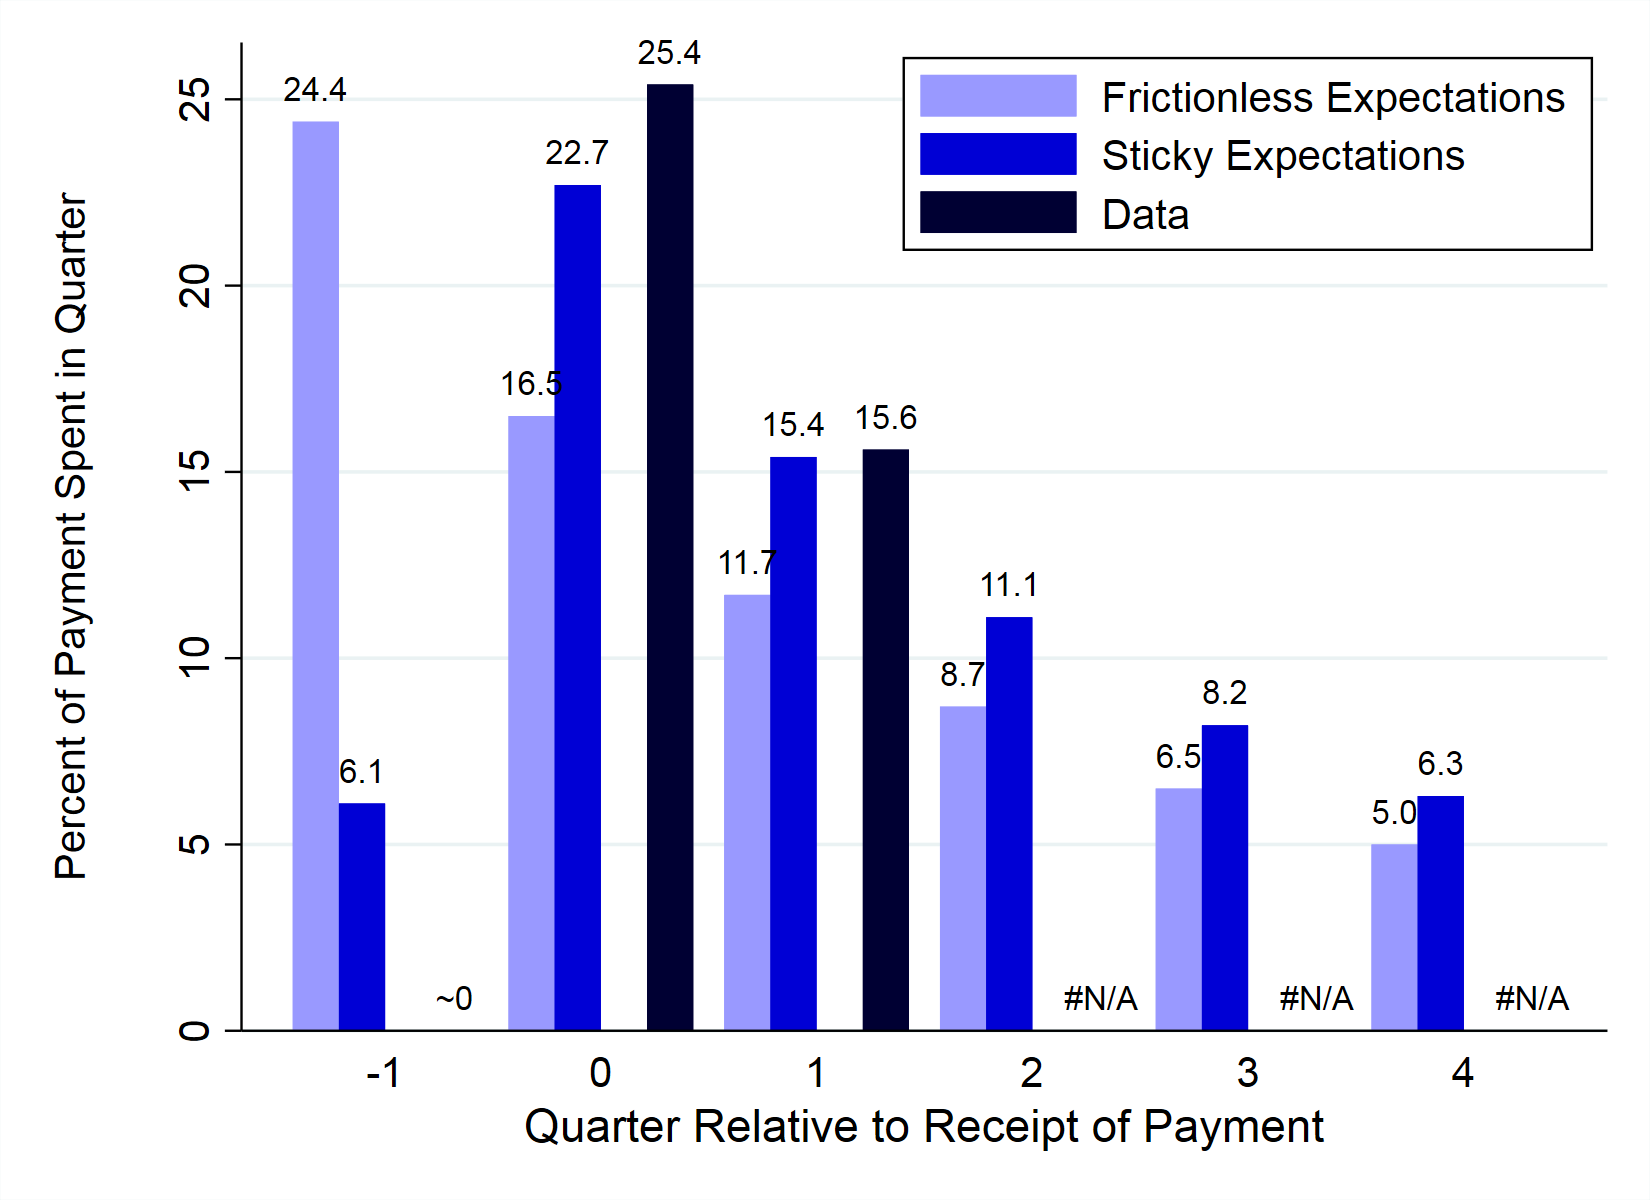
\includegraphics[width=\webWidth\textwidth]{./Figures/parkerExperiment}
    } %\end{Web}
    { 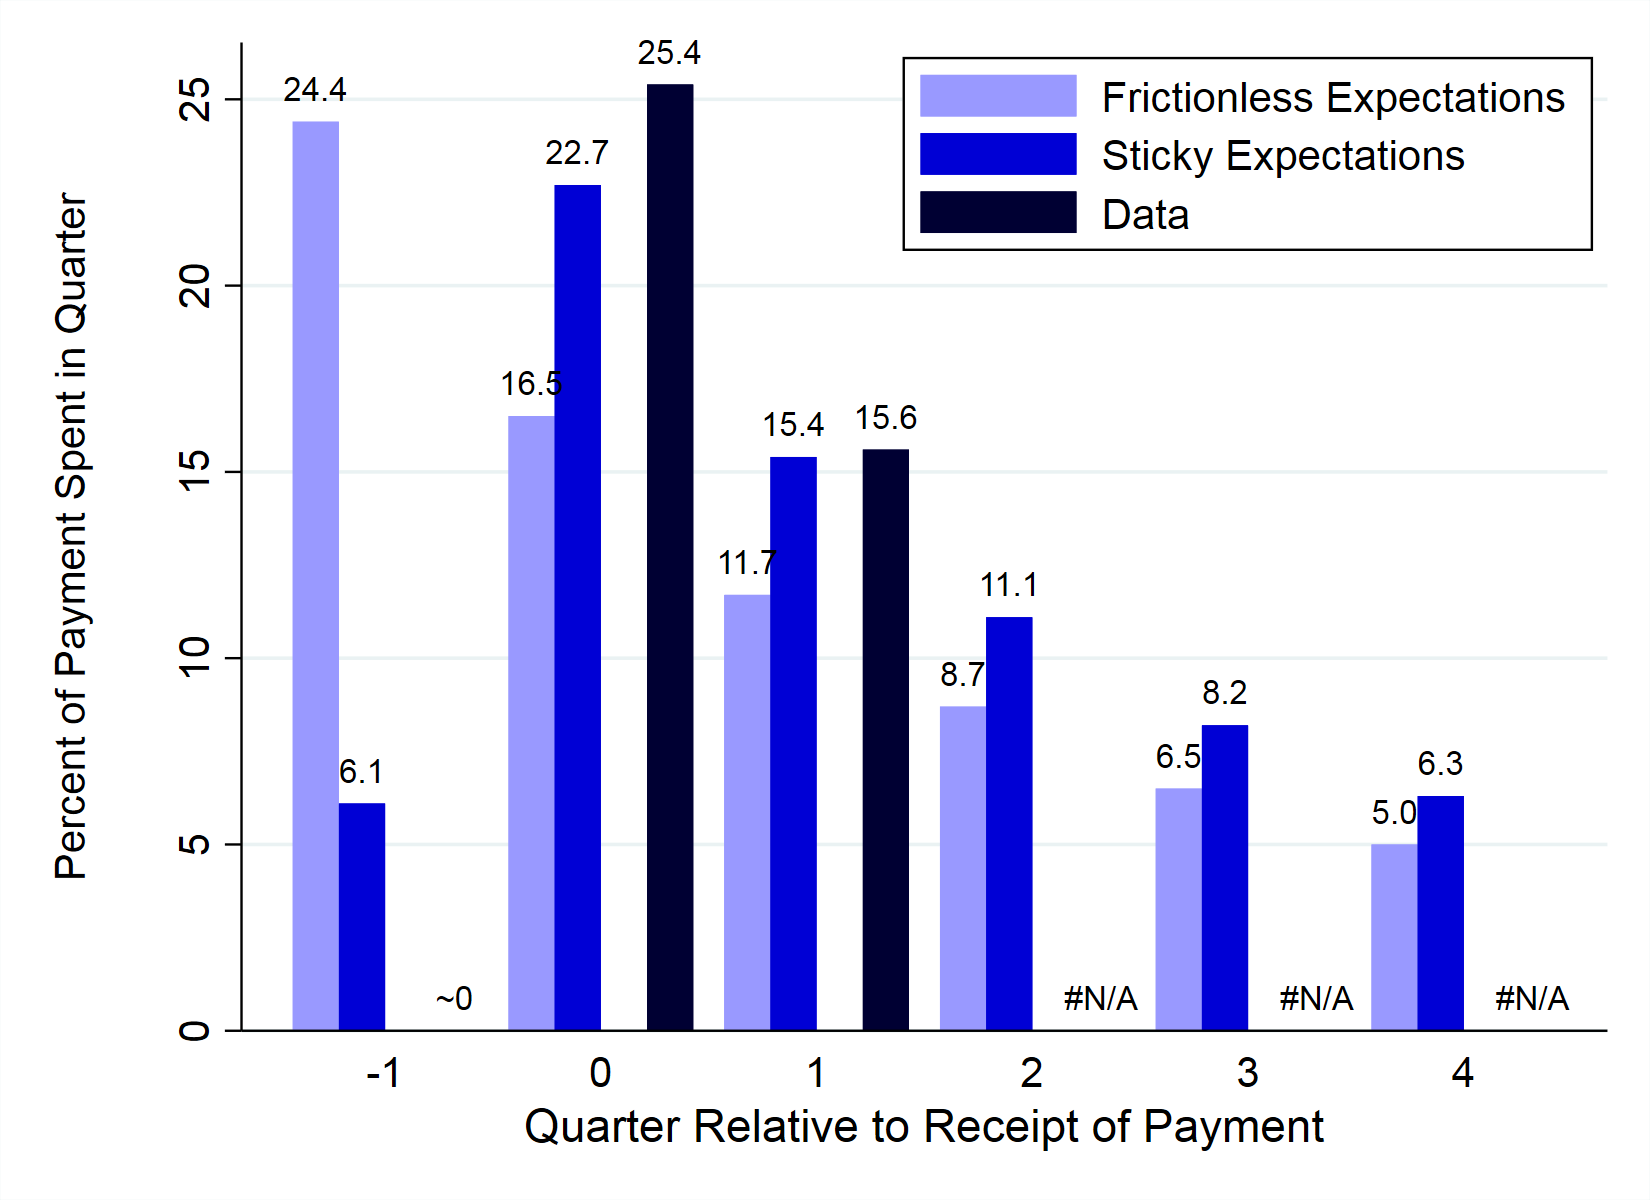
\includegraphics[width=1.0\textwidth]{./Figures/parkerExperiment}}

    \begin{flushleft}
      \footnotesize Notes: The figure shows how consumption reacts to a fiscal stimulus payment in data and in models with frictionless and sticky expectations. The evidence from data is based on \cite{psjmMPC2008}, Table ~5 and \cite{brodaParker} (the lack of reaction of consumption in quarter $-1$, ``$\sim0$'' before the payment is received). The ``\#N/A'' indicates that, to our knowledge, the literature does not estimate the reaction in quarters 2 through 4.
      \normalsize
    \end{flushleft}
  \end{figure}


  For this experiment, we employ a variant of our model that allows for ex-ante heterogeneity in households' discount factors, following \cite{cstwMPC}.\footnote{We also add unemployment insurance for this experiment.} By allowing for heterogeneity in the discount factor, we are able to calibrate the model to the distribution of wealth (and in particular the large fraction of the population with low levels of liquid wealth).  In keeping with related work by \cite{kvwWealthyH2m}, \cite{kmvHANK}, and others who emphasize the role of liquid assets, we calibrate the distribution of discount factors to match the empirical distribution of liquid wealth; \cite{cstwMPC} show that when their model is calibrated in that way, it generates an annual MPC of around 0.5.\footnote{This variant of the model produces similar results to our baseline model with respect to aggregate smoothness.\\
    An alternative approach to calibrating the distribution of $\DiscFac$ would be to target the distribution of MPCs by liquid wealth quantile, as reported for example by \cite{fhnMPC} or \cite{ckConsumption}. We also did this, but the results are too similar to the liquid wealth calibration to justify reporting.  We get similar (albeit lower) consumption responses when we calibrate the distribution of $\DiscFac$ to match the distribution of net wealth.}

  Our exact experiment is as follows.  An announcement is made in quarter $t-1$ that stimulus checks will arrive in consumers' bank accounts in period $t$.\footnote{This approximately fits the 2008 stimulus timetable. The announcement was made in February and the payments arrived between May and July. We also ran the experiment with two and three quarters advance notice and find the response on receipt of the payment remains in the right empirical range (19.9 and 16.7 percent respectively).} In line with our sticky expectation parameter, we assume 25 percent of households learn about the payment when it is announced, while the other three quarters of households are unaware until the payment arrives in period $t$. Furthermore, we assume the households who know about the upcoming payment are able to borrow against it in period $t-1$.

  The experiment sharply differentiates the models with frictionless and sticky expectations both upon announcement of the payments and when households receive the payments (Figure~\ref{parker}). Upon announcement, consumption in the frictionless model substantially increases (households spend 24.4 percent of the payment), but under sticky expectations only one quarter of households update their beliefs when the announcement is made and consumption only rises by 6.1 percent of the stimulus payment.  This small effect is in line with \cite{brodaParker}, who estimate no economically or statistically significant change in spending when the household learns that it will receive a payment.  Instead, once the stimulus payment is received, sticky expectations households substantially increase their spending---by 22.7 percent of the payment, right in the middle of the 12--30 percent range estimated in \cite{psjmMPC2008}---as three quarters of them then learn about the payment by seeing it arrive in their bank account. In contrast, in the frictionless setup the reaction of spending upon the receipt of the payment is more muted (16.5 percent).\footnote{The identification method of \cite{psjmMPC2008} retrieves the difference between households who have received the payment and those who have not. In the sticky expectations model this is 14 percent of the payment, while it is zero in the frictionless model.} In the following two quarters, consumption in the sticky expectations model is higher by 15.4 and 11.1 percent of the payment amount respectively. This also fits with the empirical evidence suggesting around 40 percent of the stimulus payment is spent in the first three quarters (\cite{psjmMPC2008}).

  The reader's intuition might have been that because our model exhibits little predictability in micro consumption growth when the consumer is experiencing ordinary income shocks (the $R^{2}$ of the predictive regression was only a few percent), and because it generates sluggishness in consumption with respect to aggregate shocks, the model would not be able to match the ample micro evidence showing high average MPCs, or the evidence from Parker and his coauthors showing that there is little ``anticipatory'' spending in advance of stimulus payments but a strong response to such payments once they have arrived.  This section shows that, in fact, the model is capable of matching the broad sweep of those micro facts, while continuing to match the aggregate excess smoothness facts.  The key is simple: In the version of our model calibrated to match high micro MPC's, people react robustly to shocks they know about, but they mostly don't know about the macro shocks until they see the money appear in their bank accounts.

